% Created 2023-08-14 lun 00:57
% Intended LaTeX compiler: pdflatex
\documentclass[9pt]{beamer}
\usepackage[utf8]{inputenc}
\usepackage[T1]{fontenc}
\usepackage{graphicx}
\usepackage{grffile}
\usepackage{longtable}
\usepackage{wrapfig}
\usepackage{rotating}
\usepackage[normalem]{ulem}
\usepackage{amsmath}
\usepackage{textcomp}
\usepackage{amssymb}
\usepackage{capt-of}
\usepackage{hyperref}
\usepackage{../modernpres}
\bibliography{../sample.bib}
\usetheme{default}
\setcounter{secnumdepth}{2}
\author{Luis Eduardo Galindo Amaya (1274895) \\
Juan Fransisco Perez Valdez  (324342)}
\date{29 de Junio 2023}
\title{Identificación y manejo de \\
material de laboratorio}
\hypersetup{
 pdfauthor={Luis Eduardo Galindo Amaya (1274895) \\
Juan Fransisco Perez Valdez  (324342)},
 pdftitle={Identificación y manejo de \\
material de laboratorio},
 pdfkeywords={},
 pdfsubject={},
 pdfcreator={Emacs 27.1 (Org mode 9.3)}, 
 pdflang={Spanish}}
\begin{document}

\maketitle

\begin{frame}[label={sec:org070d2a5}]{hola como estas}
\begin{figure}[htbp]
\centering
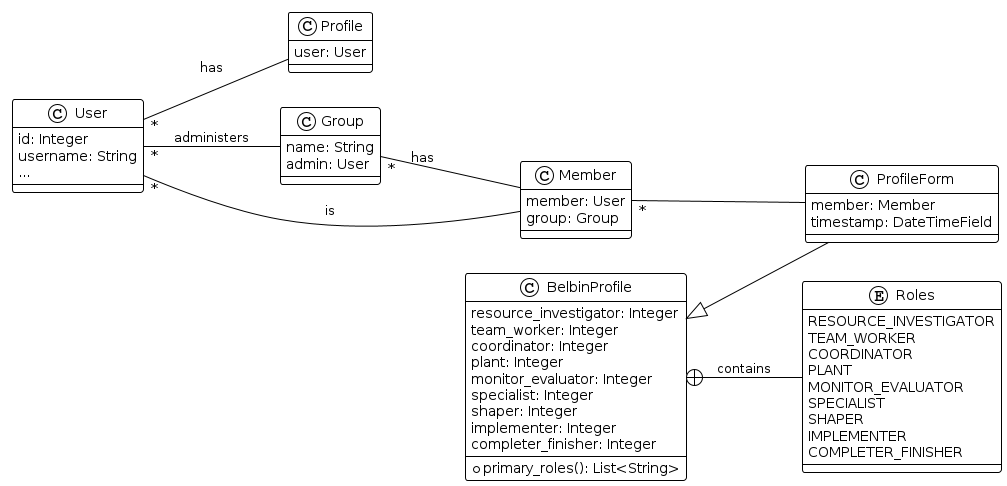
\includegraphics[width=.9\linewidth]{./a.png}
\caption{hola como estan en este dia de la vida (\cite{einstein}).}
\end{figure}
\end{frame}

\begin{frame}[label={sec:org34b459b}]{Pie de pagina}
Pellentesque dapibus suscipit ligula.  Donec posuere augue in quam.  Etiam vel
tortor sodales tellus ultricies commodo.  Suspendisse potenti.  Aenean in sem 
ac leo mollis blandit.  Donec neque quam, dignissim in, mollis nec, sagittis eu \footnote{Etiam vel tortor sodales tellus ultricies commodo} ,
\end{frame}


\begin{frame}[label={sec:org477200d}]{Listas}
\begin{block}{Hola}
\begin{itemize}
\item Como estan
\begin{itemize}
\item en este dia
\item de la lvida
\end{itemize}
\end{itemize}
\end{block}
\end{frame}

\begin{frame}[label={sec:orge091e4d},fragile]{codigo}
 \begin{verbatim}
import Yesod

data WebApp = WebApp Yesod WebApp

mkYesod "WebApp" [parseRoutes|
  / HomeR GET
|]

getHomeR = defaultLayout [whamlet|
  <div>Hello, world!
|]

main = warpEnv WebApp

\end{verbatim}
\captionof{figure}{Esta es una prueba}
\end{frame}

\begin{frame}[label={sec:orgf2dabc1}]{Tablas}
\[ \iint x^2 + y^2 - 1 \,dx \,dy \]
\begin{center}
\begin{tabular}{|l|l|}
Test 1 & Test 2\\
Hola & esta es una pruba\\
\end{tabular}

\end{center}
\end{frame}

\begin{frame}[label={sec:org6234747}]{Referencias}
\printbibliography[heading=none]
\end{frame}
\end{document}
